\documentclass[__main__.tex]{subfiles}

\begin{document}

\section{Разностные производные, их шаблоны и порядок аппроксимирования. Примеры обыкновенных центральных разностных производных 1-го и 2-го порядков. Разностные операторы и их порядок аппроксимирования, соответствующих дифференциальных операторов}

Рассмотрим банахово пространство $Y_0 = \underline{C} \left( \left[ a; b \right], \mathbb{R} \right)$, линейное многообразие $X_0 = \underline{C}^3 \left( \left[ a; b \right], \mathbb{R} \right) \subseteq Y_0$ и равномерную сетку $A = A_k = \langle a = \tau_0, \tau_1, ..., \tau_k = b \rangle$ на $\left[ a; b\right]$ шага $h = \frac{b-a}{k} \left( h \rightarrow 0 \right)$.

Пусть $f \in X_0$ и $\bar{A} \left( f \right) = {}^> y =  [ y_0 = f \left( \tau_0 \right), y_1 = f \left( \tau_1 \right), ..., y_k = f \left( \tau_k \right) \rangle \in {}^> \underline{\mathbb{R}}^{\left| A \right|} \left( A \right)$. Для узла $\tau_i \in A$ разностная формула для производной $f' \left( \tau_i \right)$ имеет вид:

\begin{equation} \label{5.1}
f' \left( \tau_i \right) = \sum_{j=0}^{k} c_j \left( h \right) f\left( \tau_j \right) + O \left( h^\alpha \right),
\end{equation}

где $h \rightarrow 0, \ c_0, c_1, ..., c_k$ - известные функции от шага $h$ и $\alpha > 0$ - порядок аппроксимирования разностной формулы $f' \left( \tau_i \right) \approx \sum_{j=0}^{k} c_j \left( h \right) f \left( \tau_i \right)$.

Не все коэффициенты $c_0, c_1, ..., c_k$ - ненулевые. Ненулевые коэффициенты наглядно иллюстрируются шаблоном Ш$\left(\tau_i\right)$ для формулы \ref{5.1}. В частности, если $0<i<k$ и $c_0 = c_1 = ... = c_{i-2} = c_{i+2} = ... = c_k = 0$,то шаблон Ш $\left( \tau_i \right)$ для такого случая показан на рисунке \ref{img_5.1}.

\begin{figure}[h!]
	\centering
	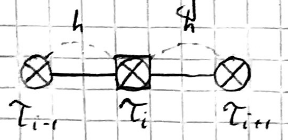
\includegraphics[width=0.3\linewidth]{img/img_5-1}
	\caption{Ш $\left( \tau_i \right)$}
	\label{img_5.1}
\end{figure}

\paragraph{Примеры}

\begin{enumerate}
	
	\item $ $
	\begin{figure}[h!]
		\centering
		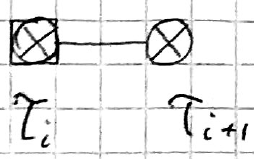
\includegraphics[width=0.3\linewidth]{img/img_5-2}
		\caption{Ш $\left( \tau_i \right)$}
		\label{img_5.2}
	\end{figure}

	Согласно такому шаблону Ш $\left( \tau_i \right)$, используя для функции f в правой окрестности узла $\tau_i$ формулу Тейлора, получаем:
	
	\begin{gather}\label{5.2}
	\begin{cases}
	f \left( \tau_i \right) = f \left( \tau_i \right) \\
	f \left( \tau_{i+1} \right) = f \left( \tau_i + h \right) = f\left( \tau_i \right) + f'\left( \tau_i \right) h + \frac{1}{2!} f''\left(\tau_i + \theta h\right) h^2
	\end{cases}
	\end{gather}
	
	где $\theta \in \left( 0; 1 \right)$.
	
	Согласно формуле \ref{5.1} и шаблону Ш $\left( \tau_i \right)$, используя \ref{5.2}, получаем: 
	
	\begin{equation}\label{5.3}
	c_i f\left( \tau_i \right) + c_{i+1} f \left( \tau_{i+1} \right) = \left( c_i + c_{i+1} \right) f \left( \tau_i \right) + c_{i+1} f' \left( \tau_i \right) h + \frac{1}{2} c_{i+1} f''\left(\tau_i + \theta h\right)h^2,
	\end{equation}
		
	где полагаем
	
	\begin{gather}\label{5.4}
	\begin{cases}
	c_i + c_{i+1} = 0 \\
	c_{i+1} = \frac{1}{h}
	\end{cases}
	\Leftrightarrow
	\begin{cases}
	c_i = - \frac{1}{h} \\
	c_{i+1} = \frac{1}{h}
	\end{cases}
	\end{gather}
	
	Согласно \ref{5.4}, формула \ref{5.3} примет вид:
	
	\begin{equation}
	\frac{1}{h} \left( f\left( \tau_{i+1}\right) - f \left( \tau_i \right)\right) = f' \left( \tau_i \right) + \frac{1}{2!} f''\left( \tau_i + \theta h \right) h \Leftrightarrow f'\left( \tau_i \right) = \frac{1}{h} \left(f\left( \tau_{i+1}\right) - f \left( \tau_i \right) \right) + O \left(h\right), h\rightarrow 0
	\end{equation}
	
	Разностную формулу $\frac{1}{h} \left( f\left( \tau_{i+1}\right) - f \left( \tau_i \right) \right)$ называют \textbf{правой разностной производной функции} f в узле $\tau_i \in A$.
	
	\item $ $
	\begin{figure}[h!]
		\centering
		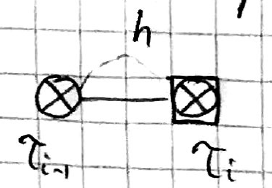
\includegraphics[width=0.05\linewidth]{img/img_5-3}
		\caption{}
		\label{img_5.3}
	\end{figure}
	Аналогично предыдущему пункту:
	
	\begin{equation}\label{5.5}
	f'\left( \tau_i \right) = \frac{1}{h} \left( f\left(\tau_i\right) - f\left( \tau_i \right) \right) + O \left( h \right), \ h \rightarrow 0
	\end{equation}
	
	- \textbf{левая разностная производная функции f в узле $\tau_i$}.
	
	\item $ $
	\begin{figure}[h!]
		\centering
		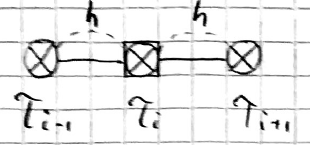
\includegraphics[width=0.05\linewidth]{img/img_5-4}
		\caption{}
		\label{img_5.4}
	\end{figure}
	
	\begin{gather}
	\begin{cases}
	f\left( \tau_{i-1} \right) = f \left( \tau_i - h \right) = f \left( \tau_i \right) - f'\left(\tau_i\right)h + \frac{1}{2!} f''\left( \tau_i \right) h^2 - \frac{1}{3!} f'''\left( \tau_i - \theta_1 h \right) h^3 \\
	f\left(\tau_i \right) = f\left(\tau_i \right) \\
	f\left( \tau_{i+1} \right) = f \left( \tau_i + h \right) = f\left( \tau_i \right) + f'\left( \tau_i \right) h + \frac{1}{2!}f''\left( \tau_i \right) h^2 + \frac{1}{3!} f'''\left( \tau_i + \theta_2 h \right)h^3
	\end{cases}
	\end{gather}
	
	Отсюда:
	
	$$
	c_{i-1} f\left( \tau_{i-1} \right) + c_i f\left( \tau_i \right) + c_{i+1} f \left( \tau_{i+1} \right) = \left( c_{i-1} + c_i + c_{i+1} \right) f \left( \tau_i \right) + \left( c_{i+1} - c_{i-1} \right) f'\left(\tau_i\right)h + \frac{1}{2!} \left(c_{i-1}+c_{i+1} \right) f''\left( \tau_i \right) h^2 +
	$$
	
	\begin{equation}\label{5.6}
	+ \frac{1}{3!} c_{i+1} f'''\left( \tau_i + \theta_2 h \right) h^3 - \frac{1}{3!}c_{i-1} f'''\left( \tau_i - \theta_1 h \right)h^3,
	\end{equation}
	
	где 
	
	\begin{gather}\label{5.7}
	\begin{cases}
	c_{i-1}+c_i+c_{i+1} = 0 \\
	c_{i-1} - c_{i+1} = \frac{1}{h}\\
	c_{i+1} + c_{i-1} = 0
	\end{cases}
	\Leftrightarrow
	\begin{cases}
	c_{i-1} = - \frac{1}{2h}\\
	c_i = 0 \\
	c_{i+1} = \frac{1}{2h}
	\end{cases}
	\end{gather}
	
	Из \ref{5.6} и \ref{5.7} получаем
	
	$$
	f'\left( \tau_i \right) = \frac{1}{2h} \left( f\left( \tau_{i+1} \right) - f \left( \tau_{i-1} \right) \right) + O \left(h^2\right), \ h\rightarrow 0
	$$
	
	 - \textbf{центральная разностная производная функции f в узле $\tau_i$}.
	 
	 \item $ $
	 
	 \begin{figure}[h!]
	 	\centering
	 	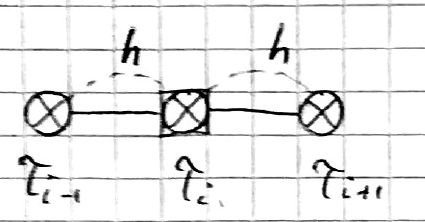
\includegraphics[width=0.4\linewidth]{img/img_5-5}
	 	\caption{}
	 	\label{img_5.5}
	 \end{figure}
	 
	 \begin{gather}
	 \begin{cases}
	 f\left( \tau_{i-1} \right) = f \left( \tau_i - h \right) = f \left( \tau_i \right) - f'\left(\tau_i\right)h + \frac{1}{2!} f''\left( \tau_i \right) h^2 - \frac{1}{3!} f'''\left( \tau_i \right) h^3 + O_1 \left(h^4\right)\\
	 f\left(\tau_i \right) = f\left(\tau_i \right) \\
	 f\left( \tau_{i+1} \right) = f \left( \tau_i + h \right) = f\left( \tau_i \right) + f'\left( \tau_i \right) h + \frac{1}{2!}f''\left( \tau_i \right) h^2 + \frac{1}{3!} f'''\left( \tau_i \right)h^3+ O_2 \left(h^4\right)
	 \end{cases}
	 \end{gather}
	
	$$
	c_{i-1} f\left( \tau_{i-1} \right) + c_i f\left( \tau_i \right) + c_{i+1} f \left( \tau_{i+1} \right) = \left( c_{i-1} + c_i + c_{i+1} \right) f \left( \tau_i \right) + \left( c_{i+1} - c_{i-1} \right) f'\left(\tau_i\right)h + \frac{1}{2!} \left(c_{i-1}+c_{i+1} \right) f''\left( \tau_i \right) h^2 +
	$$
	
	\begin{equation}
	+ \frac{1}{3!} f'''\left( \tau_i \right) \left( c_{i+1} - c_{i-1} \right) h^3 + c_{i+1} O_2 \left(h^4\right) + c_{i-1} O_1 \left( h^4 \right),
	\end{equation}
	
	где
	
	\begin{gather}
	\begin{cases}
	c_{i-1} + c_i +c_{i+1} = 0 \\
	c_{i+1} - c_{i-1} = 0 \\
	c_{i+1} + c_{i-1} = \frac{2}{h^2}
	\end{cases}
	\Leftrightarrow
	\begin{cases}
	c_{i+1}=\frac{1}{h^2}\\
	c_i = \frac{1}{h^2} \\
	c_{i-1} = - \frac{2}{h^2}
	\end{cases}
	\end{gather}
	
	$$
	f''\left( \tau_i \right) = \frac{1}{h^2} \left( f\left(\tau_{i-1}\right) - 2f \left( \tau_i \right) + f\left( \tau_{i+1} \right) \right) + O \left( h^2 \right), \ h \rightarrow 0
	$$
	
\end{enumerate}

\end{document}
